\documentclass[oneside,a4paper]{book}
\usepackage{vpcpc}
\usepackage[utf8]{inputenc}
\usepackage{ksp-lst-utf8}  % makra na listingy programov

\usepackage[absolute]{textpos}
\setlength{\TPHorizModule}{1cm}
\setlength{\TPVertModule}{\TPHorizModule}
\textblockorigin{0cm}{0cm}

\begin{document}
\mainmatter
\thispagestyle{empty}
{~}
\vspace{1cm}
\noindent
\centerline{\scalebox{4.0}{\huge\sf\bfseries VPCPC 2014~}}
\vspace{0.7cm}
\centerline{\scalebox{1.4}{\huge\sf\bfseries problems and sample solutions}}

\vfill

\begin{textblock}{10}(2,10)
\noindent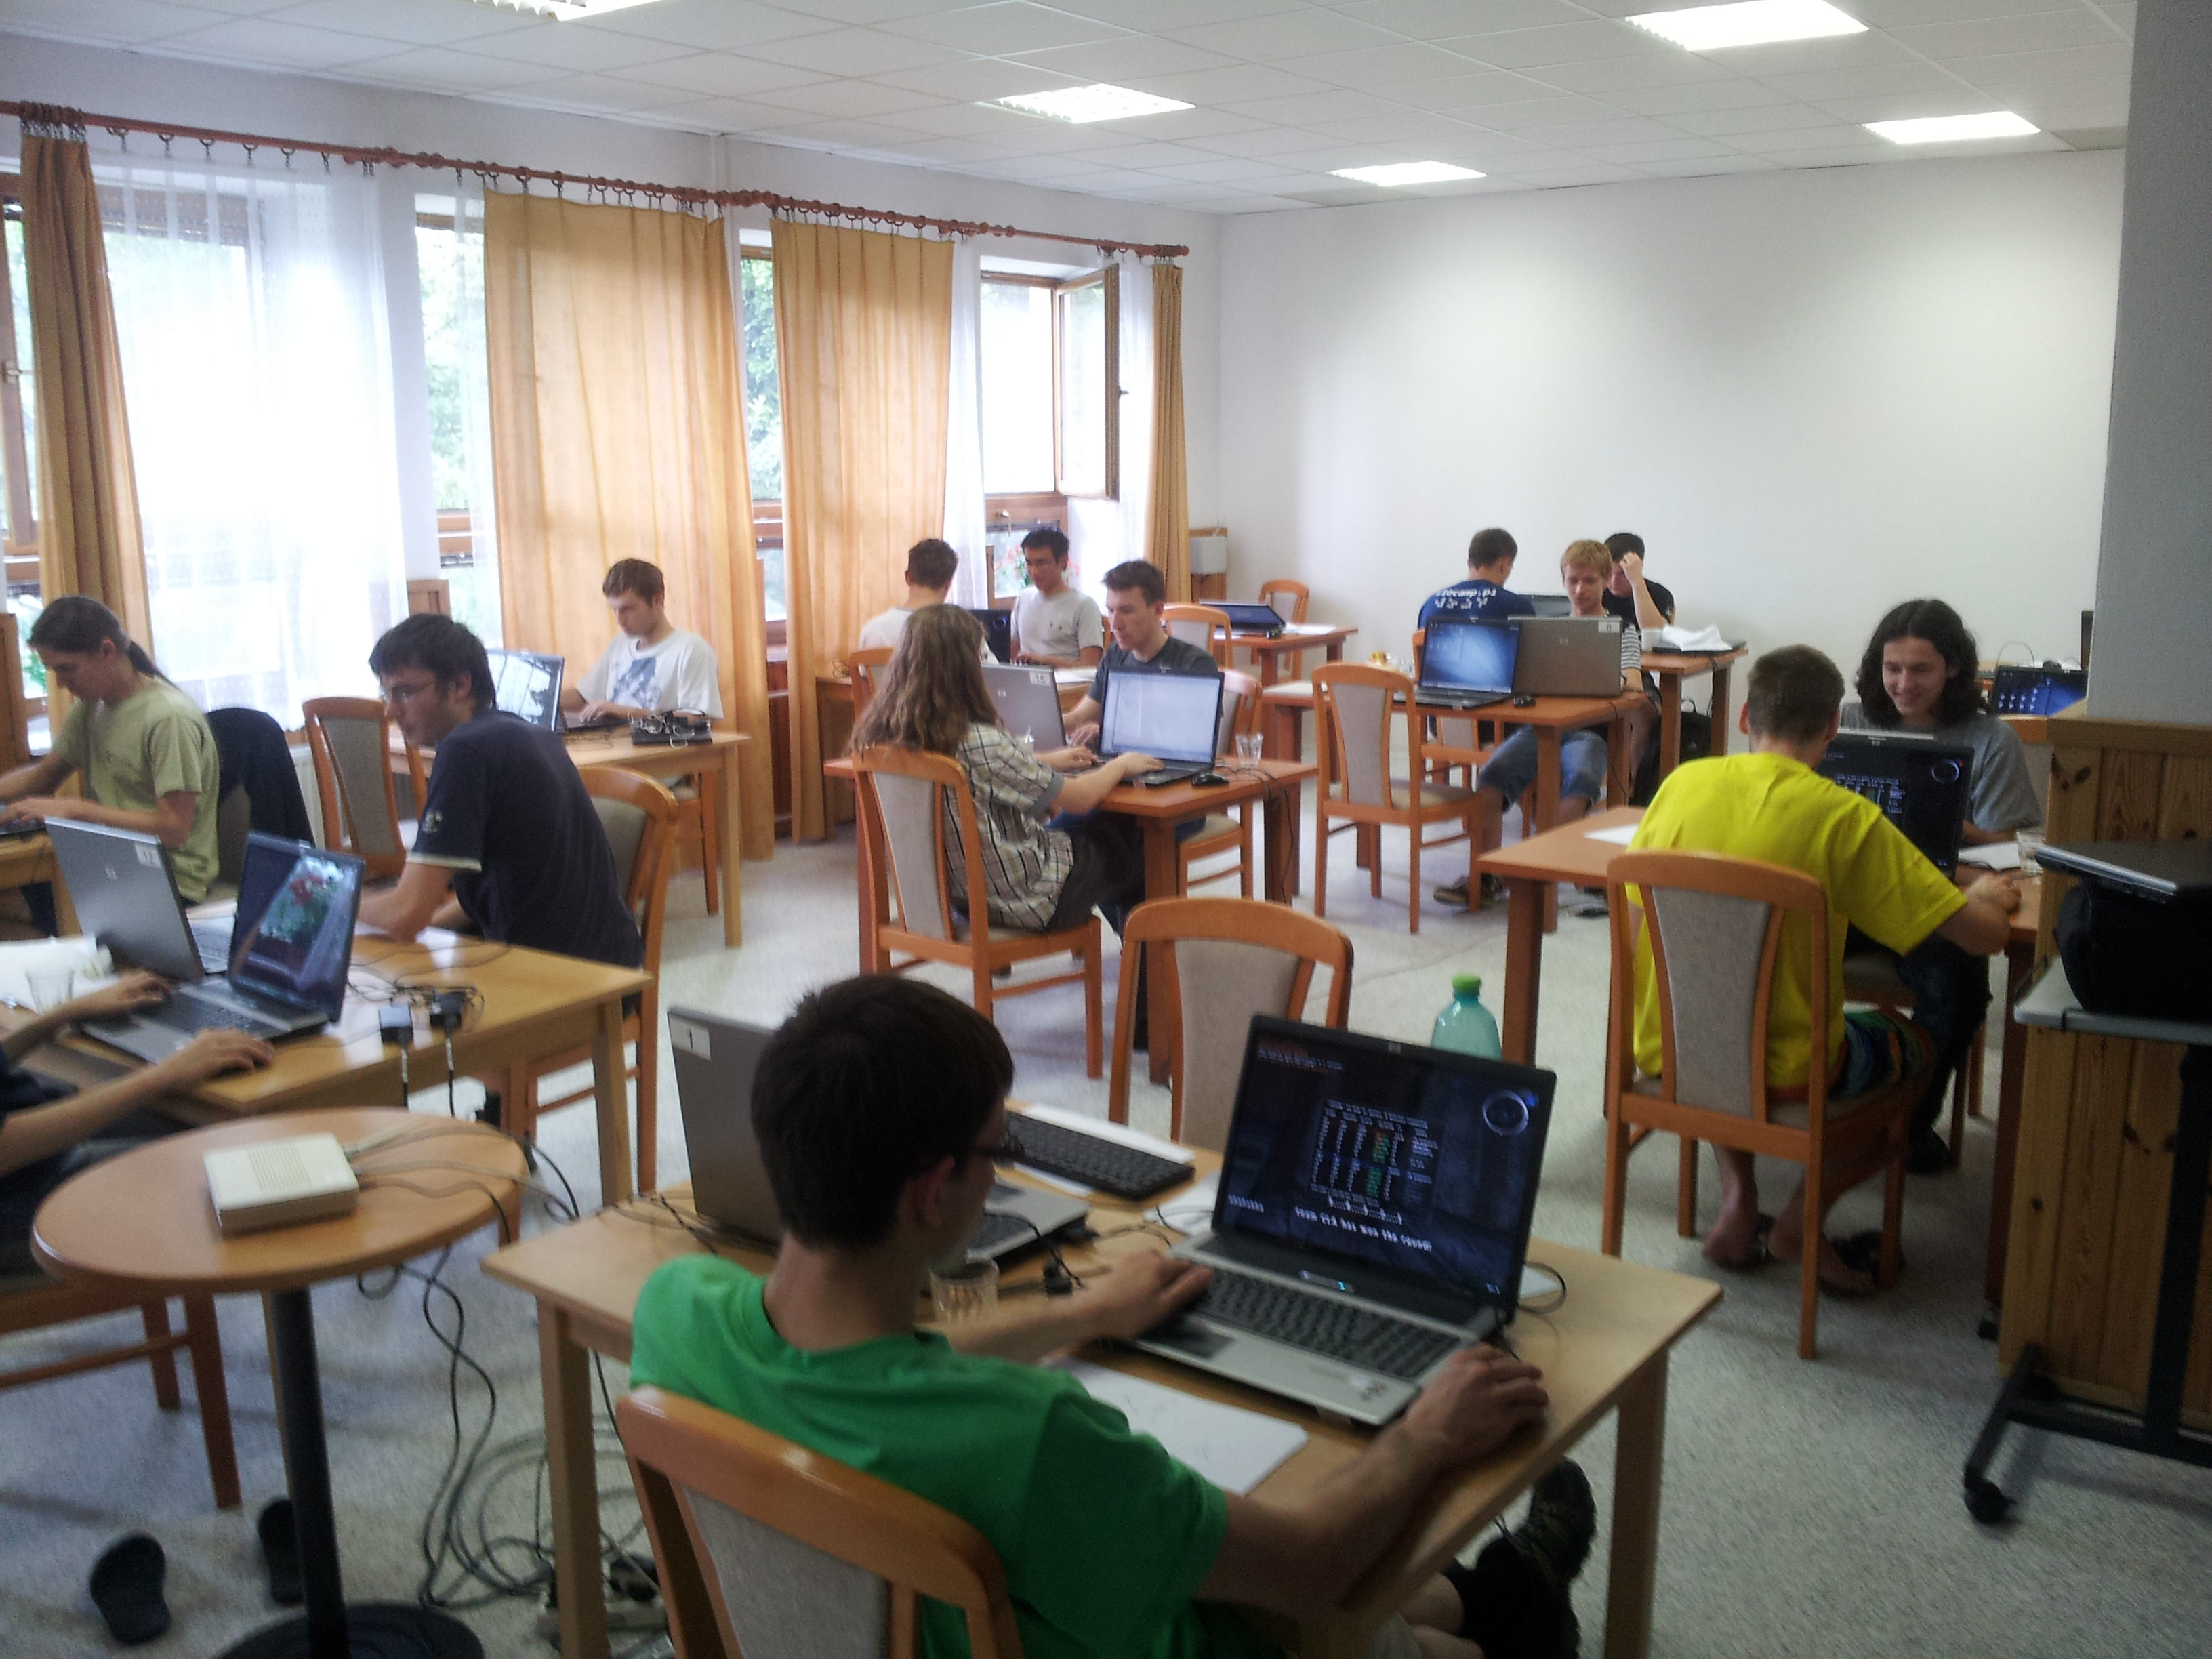
\includegraphics[height=7cm]{photos/coding.jpg}
\end{textblock}

\begin{textblock}{14}(6,16)
\noindent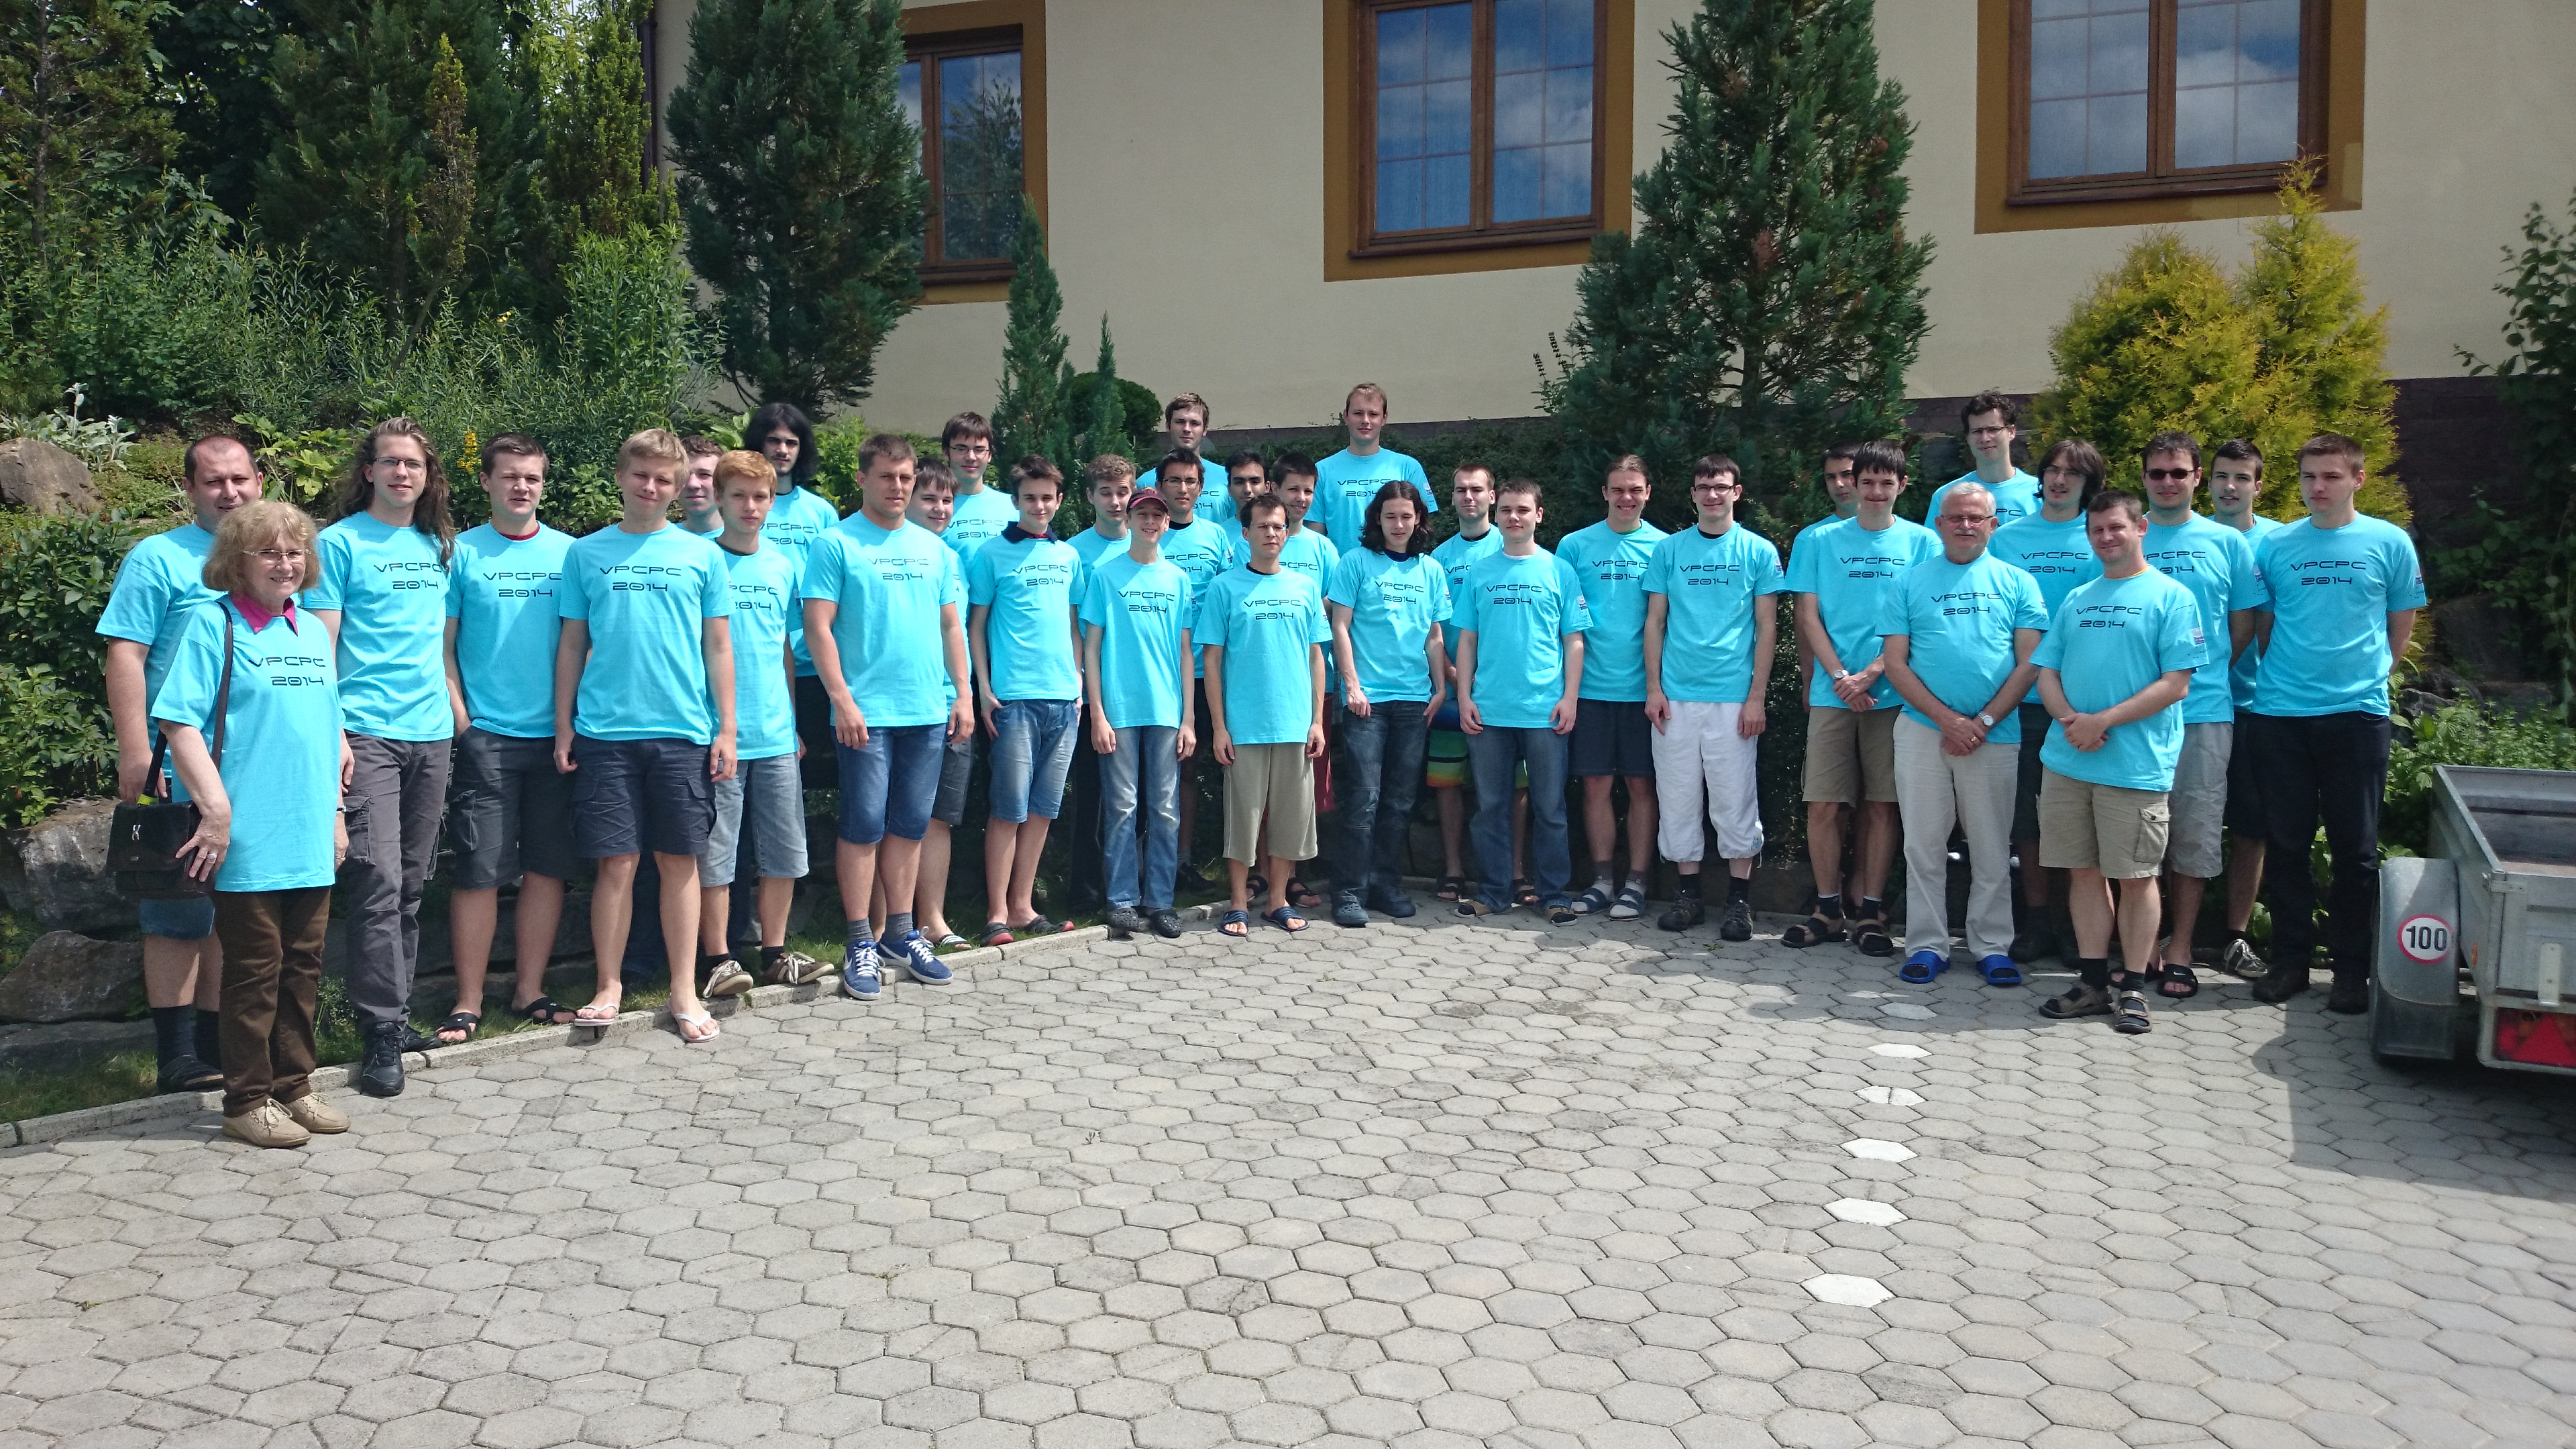
\includegraphics[height=7cm]{photos/tshirts.jpg}
\end{textblock}

\begin{textblock}{5}(12.5,11.5)
\noindent
\includegraphics[height=2.5cm]{img/vf_logo_v2.pdf}
\end{textblock}

The first ever Visegrad Programming Contests Preparation Camp took place in Danišovce, Slovakia,
between June 28th and July 6th, 2014. The camp was attended by delegations from all four Visegrad
countries: Czech Republic, Hungary, Poland, and Slovakia.
\newpage

\noindent\centerline{\sf\Large\bfseries Table of Contents}
\makeatletter\let\l@section\l@chapter\let\l@chapter\l@part\@starttoc{toc}\makeatother
\newpage

\addtocontents{toc}{\par}
\addcontentsline{toc}{chapter}{Part 0: About the camp}
\refstepcounter{section}\addcontentsline{toc}{section}{Preface}
\noindent\centerline{\sf\large\bfseries Preface}
\newpage

\refstepcounter{section}\addcontentsline{toc}{section}{Results}
\noindent\centerline{\sf\large\bfseries Results}
\bigskip

Below are the results of VPCPC 2014. Each problem was worth 100 points. 
Hence, the theoretical maximum was 2000 points: contestants could 
score at most 300 points on national days and at most 400 points
on mixed days (day 3 and day 6). Note that contestant names are
printed according to national customs -- i.e., the family name is
printed first for Hungarian contestants and last for contestants from
the other three countries.
\bigskip
\bigskip

\safeinput{results}
\newpage

\addtocontents{toc}{\par}
\refstepcounter{chapter}\addcontentsline{toc}{chapter}{Part I: Problem statements}
\refstepcounter{section}\addcontentsline{toc}{section}{Day 1: Slovak problems}
\safeinput{statements/day1-hyperways}\newpage
\safeinput{statements/day1-malloc}\newpage
\safeinput{statements/day1-shades}\newpage

\phantomsection
\refstepcounter{section}\addcontentsline{toc}{section}{Day 2: Czech problems}
\safeinput{statements/day2-buslines}\newpage
\safeinput{statements/day2-cutting}\newpage
\safeinput{statements/day2-investigation}\newpage

\refstepcounter{section}\addcontentsline{toc}{section}{Day 3: Mixed problems}
\safeinput{statements/day3-newtree}\newpage
\safeinput{statements/day3-rubik}\newpage
\safeinput{statements/day3-universities}\newpage
\safeinput{statements/day3-wall}\newpage

\refstepcounter{section}\addcontentsline{toc}{section}{Day 4: Hungarian problems}
\safeinput{statements/day4-critical}\newpage
\safeinput{statements/day4-networks}\newpage
\safeinput{statements/day4-nextperm}\newpage

\refstepcounter{section}\addcontentsline{toc}{section}{Day 5: Polish problems}
\safeinput{statements/day5-game}\newpage
\safeinput{statements/day5-posters}\newpage
\safeinput{statements/day5-sorting}\newpage

\refstepcounter{section}\addcontentsline{toc}{section}{Day 6: Mixed problems}
\safeinput{statements/day6-mission}\newpage
\safeinput{statements/day6-newspapers}\newpage
\safeinput{statements/day6-slalom}\newpage
\safeinput{statements/day6-tickets}\newpage

\addtocontents{toc}{\par}
\refstepcounter{part}
\addcontentsline{toc}{chapter}{Part II: Solutions}
\refstepcounter{section}\addcontentsline{toc}{section}{Day 1: Slovak problems}
\safeinput{solutions/day1-hyperways}\newpage
\safeinput{solutions/day1-malloc}\newpage
\safeinput{solutions/day1-shades}\newpage

\phantomsection
\refstepcounter{section}\addcontentsline{toc}{section}{Day 2: Czech problems}
\safeinput{solutions/day2-buslines}\newpage
\safeinput{solutions/day2-cutting}\newpage
\safeinput{solutions/day2-investigation}\newpage

\refstepcounter{section}\addcontentsline{toc}{section}{Day 3: Mixed problems}
\safeinput{solutions/day3-newtree}\newpage
\safeinput{solutions/day3-rubik}\newpage
\safeinput{solutions/day3-universities}\newpage
\safeinput{solutions/day3-wall}\newpage

\refstepcounter{section}\addcontentsline{toc}{section}{Day 4: Hungarian problems}
\safeinput{solutions/day4-critical}\newpage
\safeinput{solutions/day4-networks}\newpage
\safeinput{solutions/day4-nextperm}\newpage

\refstepcounter{section}\addcontentsline{toc}{section}{Day 5: Polish problems}
\safeinput{solutions/day5-game}\newpage
\safeinput{solutions/day5-posters}\newpage
\safeinput{solutions/day5-sorting}\newpage

\refstepcounter{section}\addcontentsline{toc}{section}{Day 6: Mixed problems}
\safeinput{solutions/day6-mission}\newpage
\safeinput{solutions/day6-newspapers}\newpage
\safeinput{solutions/day6-slalom}\newpage
\safeinput{solutions/day6-tickets}\newpage

\end{document}
